\subsection{Упражнение 1}

Скачайте с сайта http://freesound.org , включающий музыку, речь или иные звуки, имеющие четко выраженную высоту. Выделите примерно полусекундный сегмент, в котором высота постоянна. Вычислите и распечатайте спектр выбранного сегмента. Как связаны тембр звука и гармоническая структура, видимая в спектре?


\noindent Используйте high\_pass, low\_pass, и band\_stop для фильтрациитех или иных гармоник. Затем преобразуйте спектры обратно в сигнал и прослушайте его. Как звук соотносится с изменениями, сделанными в спектре?
    

Загружаем звуки игры на пианино, взятые на сайте freesound.org и загруженные на мой репозиторий, после читаем звуки в специальный Wave класс и вырезаем фрагмент.

\begin{lstlisting}[language=Python]
if not os.path.exists('469283__matt141141__cm7-dm7-115bpm-loop.wav'):
    !wget https://github.com/sergeyfedorov02/Telecom/raw/main/469283__matt141141__cm7-dm7-115bpm-loop.wav

wave = read_wave('469283__matt141141__cm7-dm7-115bpm-loop.wav')

wave.make_audio()
\end{lstlisting}

Построим график wave
\begin{lstlisting}[language=Python]
wave.plot()
decorate(xlabel='Time (s)')
\end{lstlisting}

\begin{figure}[H]
	\begin{center}
		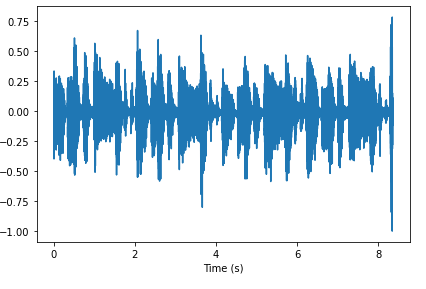
\includegraphics[scale=1]{fig/lab01/lab01_01.png}
		\caption{График всего звука}
	\end{center}
\end{figure}

Выделим полусекундный фрагмен, в котором высота постоянна и построим его график
\begin{lstlisting}[language=Python]
segment = wave.segment(start=5.2, duration=0.5)
segment.make_audio()

segment.plot()
decorate(xlabel='Time (s)')
\end{lstlisting}

\begin{figure}[H]
	\begin{center}
		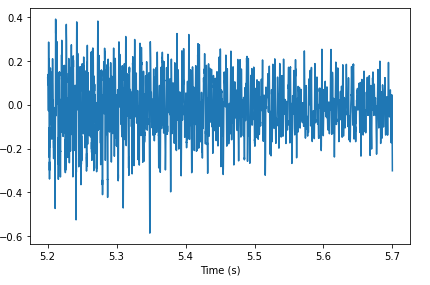
\includegraphics[scale=1]{fig/lab01/lab01_02.png}
		\caption{График сегмента звука}
	\end{center}
\end{figure}

Спектр сегмента
\begin{lstlisting}[language=Python]
spectrum = segment.make_spectrum()
spectrum.plot(high=5000)
decorate(xlabel='Frequency (Hz)')
\end{lstlisting}

\begin{figure}[H]
	\begin{center}
		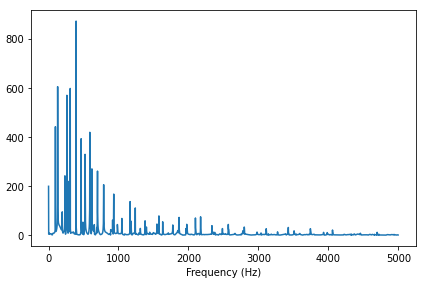
\includegraphics[scale=1]{fig/lab01/lab01_03.png}
		\caption{Спектр сегмента звука}
	\end{center}
\end{figure}

Осуществим фильтрацию при помощи специальных функций

Уберем частоты ниже 450
\begin{lstlisting}[language=Python]
spectrum.high_pass(450)
spectrum.plot(high=5000)
decorate(xlabel='Frequency (Hz)')
\end{lstlisting}

\begin{figure}[H]
	\begin{center}
		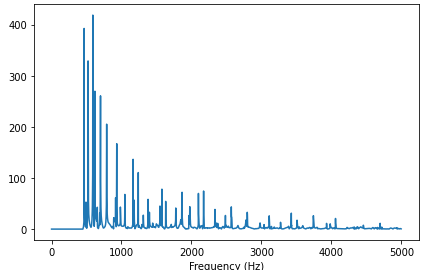
\includegraphics[scale=1]{fig/lab01/lab01_04.png}
		\caption{График частот без тех, что ниже 450}
	\end{center}
\end{figure}

Уберем частоты выше 2000
\begin{lstlisting}[language=Python]
spectrum.low_pass(2000)
spectrum.plot(high=5000)
decorate(xlabel='Frequency (Hz)')
\end{lstlisting}

\begin{figure}[H]
	\begin{center}
		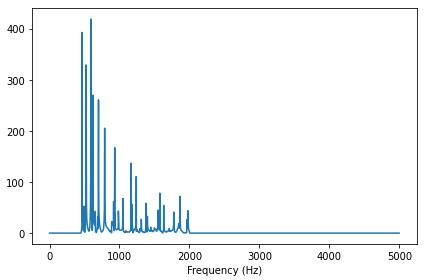
\includegraphics[scale=1]{fig/lab01/lab01_05.png}
		\caption{График частот без тех, что выше 2000}
	\end{center}
\end{figure}

Применим ФПЗ, чтобы убрать частоты в срезе
\begin{lstlisting}[language=Python]
spectrum.band_stop(500, 1100)
spectrum.plot(high=5000)
decorate(xlabel='Frequency (Hz)')
\end{lstlisting}

\begin{figure}[H]
	\begin{center}
		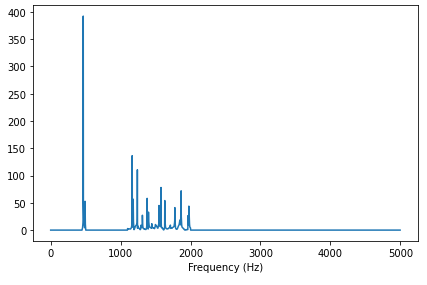
\includegraphics[scale=1]{fig/lab01/lab01_06.png}
		\caption{График частот после применения ФПЗ}
	\end{center}
\end{figure}

Преобразуем спектр обратно в сигнал
\begin{lstlisting}[language=Python]
test = spectrum.make_wave()
test.plot()
decorate(xlabel='Time (s)')
\end{lstlisting}

\begin{figure}[H]
	\begin{center}
		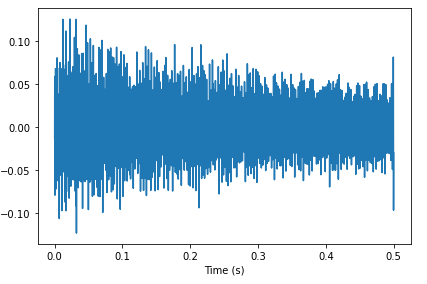
\includegraphics[scale=1]{fig/lab01/lab01_07.png}
		\caption{График преобразованного сигнала}
	\end{center}
\end{figure}

Проведем сравнение изначального среза и отфильтрованного

Изначальный:
\begin{lstlisting}[language=Python]
segment.make_audio()
\end{lstlisting}

Отфильтрованный:
\begin{lstlisting}[language=Python]
segment.make_audio()
\end{lstlisting}

Можно сделать вывод, что отфильрованный звук лишен объема (получился "плоский" звук)


\subsection{Упражнение 2}

Создайте сложный сигнал из объектов SinSignal и CosSignal, суммируя их. Обработайте сигнал для получения wave и прослушайте его. Вычислите Spectrum и распечатайте. Что произойдёт при добавлении частотных компонент, не кратных основным?

Создадим сложный сигнал из объектов SinSignal и CosSignal, суммируя их
\begin{lstlisting}[language=Python]
cos_sig = CosSignal(freq=300, amp=1.2, offset=0)
sin_sig = SinSignal(freq=100, amp=0.4, offset=0)
sin_sig2 = SinSignal(freq=700, amp=0.1, offset=0)
m_sig = cos_sig + sin_sig + sin_sig2
\end{lstlisting}

Построим график суммы
\begin{figure}[H]
	\begin{center}
		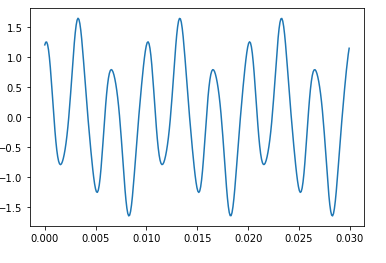
\includegraphics[scale=1]{fig/lab01/lab01_08.png}
		\caption{Графиксуммы сигналов}
	\end{center}
\end{figure}

Сделаем wave и послушаем
\begin{lstlisting}[language=Python]
wave = m_sig.make_wave()

wave.make_audio()
\end{lstlisting}

Вычислим спектр
\begin{lstlisting}[language=Python]
spectrum = wave.make_spectrum()
spectrum.plot()
\end{lstlisting}

\begin{figure}[H]
	\begin{center}
		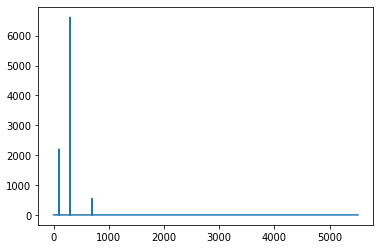
\includegraphics[scale=1]{fig/lab01/lab01_09.png}
		\caption{Спектр сигнала}
	\end{center}
\end{figure}

Теперь добавим частотный компонент, не кратный основным
\begin{lstlisting}[language=Python]
wave_2 = (m_sig + CosSignal(freq=550, amp=0.66, offset=0)).make_wave()
wave_2.make_audio()

wave_2.make_spectrum().plot()
\end{lstlisting}

\begin{figure}[H]
	\begin{center}
		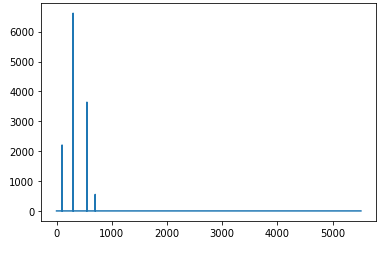
\includegraphics[scale=1]{fig/lab01/lab01_10.png}
		\caption{График после добавления частотного компонента}
	\end{center}
\end{figure}

Звук перестал быть однотонным


\subsection{Упражнение 3}

Напишите функцию strech, берущую wave и коэффицент изменения. Она должна ускорять или замедлять сигнал изменением ts и framerate.

Создадим функцию stretch, которая будет замедлять или ускорять сигнал в зависимости от коэффициента измнения
\begin{lstlisting}[language=Python]
def stretch(wave, coef):
  wave.ts *= coef
  wave.framerate /= coef
  
wave = read_wave('469283__matt141141__cm7-dm7-115bpm-loop.wav')
wave.make_audio()
\end{lstlisting}

Проверим замедление в 2 раза
\begin{lstlisting}[language=Python]
slow_wave = wave
stretch(slow_wave, 2)
slow_wave.make_audio()
\end{lstlisting}

Исходя из результатов видно, что звук замедлился в 2 раза, так как длинна дорожки в секундах, стала в 2 раза дольше

Проверим ускорение в 2 раза
\begin{lstlisting}[language=Python]
fast_wave = wave
stretch(fast_wave, 0.5)
fast_wave.make_audio()
\end{lstlisting}

Исходя из результатов видно, что звук ускорился в 2 раза, так как длинна дорожки в секундах, стала в 2 раза меньше


\subsection{Вывод}
В ходе данной работы было выполнено знакомство с основыми понятиями при работе со звуками и сигналами. При помощи библиотеки thinkDSP открывается множество возможностей по взаимодействию с сингалами, таких как их созданию, так и для их обработки